\chapter{6DoF Pose Tracking in Planar Scenes}
\label{sec:planar_scenes}

Throughout this work the following notation is employed: $W$ denotes
the world frame, $C_1$ or $C_2$ denotes a camera frame.  $T_{AB}$ is
the transformation from frame $A$ to frame $B$, measured in frame $A$.

$\vec{X}$ the position of the event with respect to world or camera
frame, $\vec{x}$ the calibrated coordinates of the event.

\section{From Events to Frame}
\label{sec:event_warp}
We group a set of events $\mathscr{E}\doteq \{e_k\}_{k=1}^N$ into a
temporal window, optimize the motion and scene parameters within this
window, then shift the window to the next set of events and repeat
this process. The temporal window size is defined by the event numbers
$N$, which should be chosen small enough so that a constant velocity
model could be applied within this window. We choose event numbers
against a fixed time interval to define the window size, because this
corresponds to the data-driven nature of an event-based camera: the
more rapid the apparent motion of the scene is, the larger the event
rate will be. If the scene stops moving, no events will be generated,
the pose will also not be further updated.

An event frame is thus formed by summing up events within this
window. If we simply sum along the time axis, the intensity at each
pixel will be the sum of the polarities of all the events that are
triggered at this pixel location within the window
\begin{equation}
  \label{eq:intensity}
  \mathcal{I}(\vec{x}) = \sum_{k=1}^N\pm_k\delta(\vec{x}-\vec{x}_k),
\end{equation}
with $\pm_k$ and $\vec{x}_k$ denoting the polarity and pixel
coordinates of the $k$th event, respectively. After warping the events
with $\vec{x}'_k=\mat{W}(\vec{x}_k,t;\theta)$, we substitute
$\vec{x}_k$ in the above equation to $\vec{x}'_k$.

\subsection{Measuring the Sharpness of an Image}
\label{sec:contrast}
There are several metrics one could choose from to measure the
contrast of an image. A local contrast metric could be, for example,
convoluting the image with a high pass filter
\begin{equation}
  \label{eq:high_pass_filter}
  \mathcal{C}_H=
  \begin{bmatrix}
    -1&-1&-1\\
    -1&8&-1\\
    -1&-1&-1
  \end{bmatrix},
\end{equation}
and sum the pixel value of the filtered image. However, this metric
only compare a pixel with its 8 neighbors, thus an image with
scattered events (large noise) is also a valid configuration, as shown
in \cref{fig:contrast}(a). The Michelson contrast
\citep{michelson1995studies}, defined as
$\mathcal{C}_M=\left(\mathcal{I}_{\mathrm{max}}-\mathcal{I}_{\mathrm{min}}\right)/\left(\mathcal{I}_{\mathrm{max}}+\mathcal{I}_{\mathrm{min}}\right)$,
only considers the highest and lowest luminance in the image and is
thus more suitable to quantify contrast for periodic functions.

We choose to measure the contrast by the variance of the image,
defined by

\begin{equation}
  \label{eq:variance}
  \mathrm{Var}\left(\mathcal{I}\left(\vec{x};\bm{\theta}\right)\right)\doteq\frac{1}{\mid\Omega\mid}\int_{\Omega}\left(\mathcal{I}\left(\vec{x};\bm{\theta}\right)-\mu\left(\mathcal{I}\left(\vec{x};\bm{\theta}\right)\right)\right)^2d\vec{x},
\end{equation}
where $\mu\left(\mathcal{I}\left(\vec{x};\bm{\theta}\right)\right)$ is the average
image intensity. Since our goal is to align events triggered from the
same visual stimuli, the variance would be a very suitable metric, as
a squared metric favors the configuration that projects as many events
as possible to the same pixel.

Intergral sum pixels

\begin{figure}
  \begin{minipage}[t]{0.48\textwidth}
    \centering 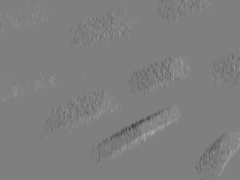
\includegraphics[width =
    \textwidth]{images/high_pass_contrast.png}
    % \label{subfig:texture}
    (a) An optimized frame using sharpening filter metric
  \end{minipage}
  \hfill
  \begin{minipage}[t]{0.48\textwidth}
    \centering 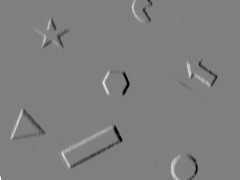
\includegraphics[width =
    \textwidth]{images/variance_contrast.png}
    % \label{subfig:map}
    (b) An optimized frame using variance metric
  \end{minipage}
  \caption{Comparison between two different metrics}
  \label{fig:contrast}
\end{figure}



\subsection{Planar Homography}

\label{sec:planar_homo}
The warp function $\vec{x}'=\mat{W}(\vec{x},t;\bm{\theta})$ does not only
depend on the motion parameters, but also the scene parameters, which
is the unknown depth.  In the case of a planar scene the problems
simplifies, since a plane $\mathbf{P}$ can be parameterized by two
sets of parameters: $\vec{n}\in\mathbb{S}^2$ the unit surface normal
of $\mathbf{P}$ with respect to the current camera frame, and $d$ the
distance from the camera center to $\mathbf{P}$. The warp function
then becomes
\begin{align}
  \vec{X}'=&\mat{R}(t)\vec{X}+\vec{T}(t)\\
  \vec{X}=&\mat{R}(t)^\top\left(\vec{X}'-\vec{T}(t)\right)\\
  \vec{X}=&\mat{R}(t)^\top\left(\mat{I}+\vec{T}(t)\vec{n}^\top/d\right)\vec{X}',  \label{eq:planar_homo_0}
\end{align}
thus
$\vec{x}'\sim\left(\mat{R}(t)^\top\left(\mat{I}+\vec{T}(t)\vec{n}^\top/d\right)\right)^{-1}\vec{x}$.
Here $(\mat{R}(t), \vec{T}(t))\in SE(3)$ denotes the relative pose
between two cameras at which the current event being warped and the
first event within the window happened, and $t$ is the relative
timestamp with respect to the first event. Under a constant velocity
model with linear velocity $\vec{v}\in\mathbb{R}^3$ and angular
velocity $\bm{\omega}\in\mathbb{R}^3$, the translation is given by
\begin{equation}
  \label{eq:translation}
  \vec{T}(t)=\vec{v}t,
\end{equation}
the rotation matrix is given by the \textit{exponential map} exp:
$\mathfrak{so}(3)\rightarrow SO(3)$:
\begin{equation}
  \label{eq:rotation}
  \mat{R}(t)=\mathrm{exp}(\bm{\omega}^\wedge t),
\end{equation}
where $^\wedge$ is the \textit{hat} operator
\begin{equation}
  \label{eq:hat}
  \bm{\omega}^\wedge=
  \begin{bmatrix}
    \omega_1\\\omega_2\\\omega_3
  \end{bmatrix}
  =
  \begin{bmatrix}
    0&-\omega_3&\omega_2\\
    \omega_3&0&-\omega_1\\
    -\omega_2&\omega_1&0
  \end{bmatrix}
  \in\mathfrak{so}(3).
\end{equation}

\section{From Frames to Map}
\label{sec:frame2map}
The contrast maximization procedure in the above section optimizes the
relative pose between successive frames. We show in this section that
the same idea can be applied to perform global pose tracking in planar
scenes. We first explain how the map is defined, and how to track a
known map, then we shown how this map is built by selecting a set of
keyframes.

\subsection{Map}
\label{sec:map}
A map is a plane with three components: the normal direction
$\vec{n}_w$, the distance $d_w$ to the origin, and the texture; the
texture of a map represents all the edges on the plane. \Cref{fig:map}
shows the an example of such map. \Cref{fig:map}(a) also shows the set
of keyframes used to construct the map. We will talk more about
keyframes in \cref{sec:keyframe2map}. The global coordinate is chosen
as the camera coordinate of the first frame.

\begin{figure}
  \begin{minipage}[t]{0.48\textwidth}
    \centering 
\includegraphics[width =
    \textwidth]{images/map_805.jpg}
    % \label{subfig:texture}
    (a) The texture of a map
  \end{minipage}
  \hfill
  \begin{minipage}[t]{0.48\textwidth}
    \centering 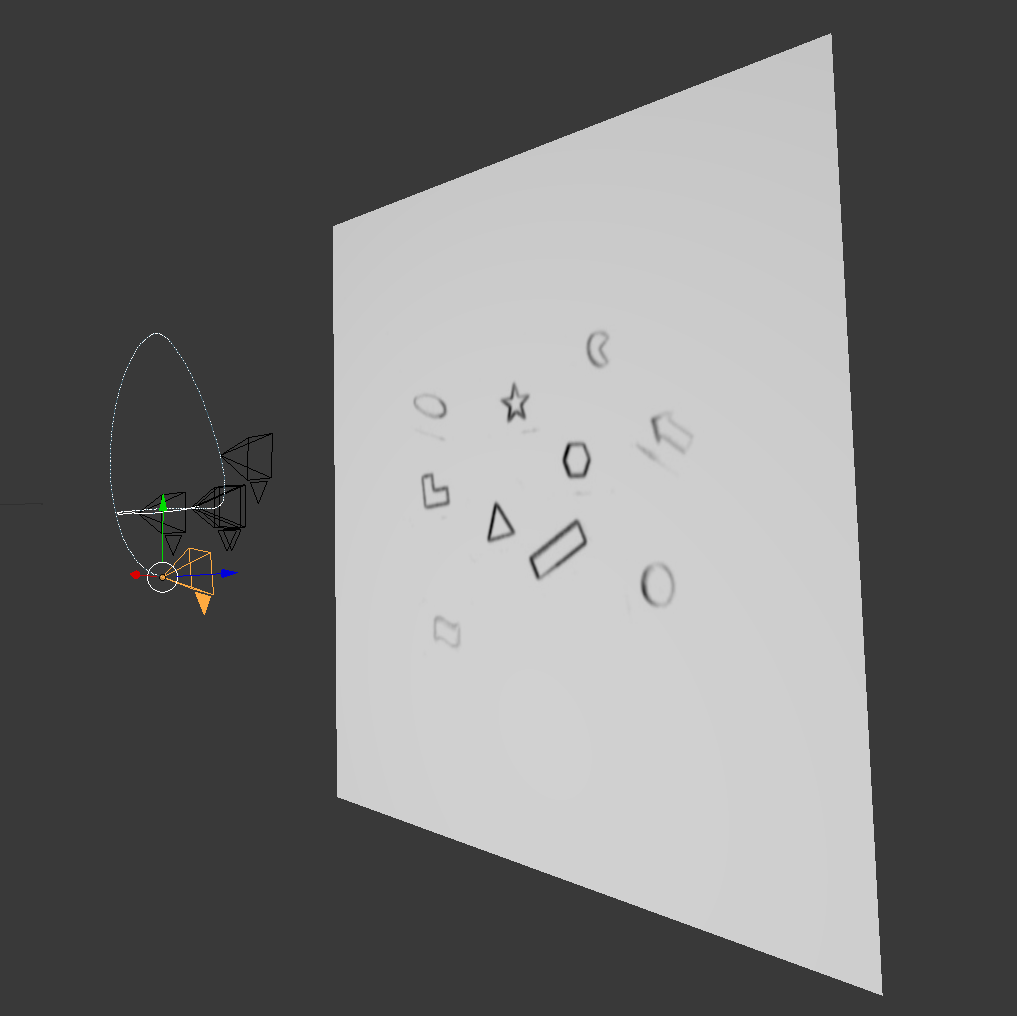
\includegraphics[width = \textwidth]{images/4.png}
    % \label{subfig:map}
    (b) A map in the global frame
  \end{minipage}
  \caption{Map}
  \label{fig:map}
\end{figure}



\subsection{Tracking}
\label{sec:tracking}
Suppose a map is present, then the normal direction $\vec{n}_w$ of the
plane and the distance $d_w$ to the origin are known. Also the pose of
the current frame $(\mat{R}_{wc}, \vec{T}_{wc})\in SE(3)$ is
determined by the motion estimation from the last frame (a quick note
to the terminology we are using: whenever we say the \textit{pose} of
a frame, we always refer to the camera \textit{pose} at which the
first event within the frame happens). The parameters left to be
estimated for each frame is
$\phi=\left(\bm{\omega},\vec{v}\right)\in\mathbb{R}^6$. By
substituting $\vec{n}$ with $\vec{n}_c = \mat{R}_{cw}\vec{n}_w$, and
$d$ with $d_c = d_w+\vec{T}_{wc}\cdot\vec{n}_w$ in
\cref{eq:planar_homo_0}, we get the homography matrix within each
frame as
\begin{equation}
  \label{eq:planar_homo_1}
  \mat{H}_1=\mat{R}^\top\left(\mat{I}+\vec{T}\vec{n}_c^\top/d_c\right)
\end{equation}
and $\vec{x}'_c\sim\mat{H}_1^{-1}x_c$.

A nonlinear optimizing problem naturally suffers from local
optima. Without a good initialization, the motion computed with the
method in \cref{sec:event_warp} could sometimes be a local optimum
delivering an image that appears sharp, despite being wrongly
estimated (see \cref{fig:local_optimum}). In order to make sure that
the estimated motion from the per frame contrast maximization also
conform to the global map. Thus we perform another optimization, where
we project the events of the current frame to the global map. The
parameter set is still $\left(\bm{\omega}^\top,\vec{v}^\top\right)$,
and we use the output from last procedure as an initial guess.

The procedure described in the first paragraph of this section can be
understood as projecting the events on a \textit{blank
  canvas}. Similarly, in the projecting-to-map procedure we project
the events on the \textit{texture} of the map, and measure the
strength of the synthesized image with the same variance function as
in \cref{eq:variance}, thus finding the set of the parameters that
best align the events in the current frame to their correspondences in
the texture.

The projection from an event to the map is
\begin{equation}
  \label{eq:frame2map}
  \vec{x}_w \sim \mat{R}_n\mat{H}_2^{-1}\mat{H}_1^{-1}\vec{x}_c,
\end{equation}
with $\mat{R}_n$ the transformation from the orientation of the global
frame to the orientation of the map, computed by
\begin{align}
  \mat{K}& =(\vec{n}_w\times \vec{z})^\wedge\\
  \mat{R}_n&=\mat{I} +\mat{K} + \mat{K}^2/ (1 +  \vec{n_w}\cdot\vec{z}),  \label{eq:global2map}
\end{align}
where $\vec{z}=(0,0,-1)$ denotes the plane fronto-parallel to the
camera, and
\begin{equation}
  \label{eq:frame2global}
  \mat{H}_2 = \mat{R}_{cw}\left(\mat{I} + \vec{T}_{wc}\vec{n}^\top/d_w\right)
\end{equation}
is the projection from the current frame to the global frame, with
$\mat{R}_{wc}, \mat{T}_{wc}$ being the pose of the current
frame. $\mat{H}_1$ is the planar homography for each frame as in
\cref{eq:planar_homo_1}. But the $\mat{R}(t)$ and $\vec{T}(t)$ might
be different since we are refining these parameters.

After projecting, we obtain an image composed of the map texture and
the events of the current frame. We maximize the contrast of this
image using the cost function defined in \cref{eq:variance}. The
optimized velocity is used for propagating the pose to the next
incoming frame via
\begin{align}
  \label{eq:pose_propagation}
  \vec{T}_{wc_2}&=\mat{R}_{wc_1}\vec{v}\Delta t+ \vec{T}_{wc_1}\\
  \mat{R}_{wc_2}& =\mat{R}_{wc_1}\mathrm{exp}(\bm{\omega}^\wedge \Delta t),
\end{align}
where $c_1$ and $c_2$ denotes the current frame and the next frame,
respectively, and $\Delta t$ is the temporal size of the current
frame.

\begin{figure}
  \begin{minipage}[t]{0.48\textwidth}
    \centering 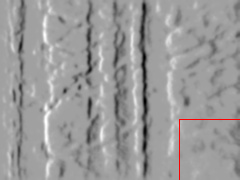
\includegraphics[width =
    \textwidth]{images/slider_estimation.png}
    \label{subfig:estimation}
    (a) Estimation
  \end{minipage}
  \hfill
  \begin{minipage}[t]{0.48\textwidth}
    \centering 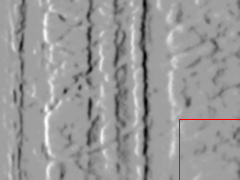
\includegraphics[width =
    \textwidth]{images/slider_groundtruth.png}
    \label{subfig:groundtruth}
    (b) Groundtruth
  \end{minipage}
  \hfill

  \begin{minipage}[t]{\textwidth}
    \centering 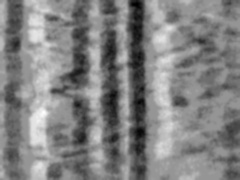
\includegraphics[width =
    0.48\textwidth]{images/slider_zero_motion.jpg}
    \label{subfig:estimation}
    \\(c) Without motion compensation
  \end{minipage}
  \hfill

  \caption{An example of local optima. This is the dataset
    \textit{slider\_hdr\_close} with a window size of 50000
    events. (a) shows the optimized image with \textit{linear
      velocity} $( 0.231, 0.109, 0.256)$, \textit{angular velocity}
    $(0.405, -0.130, -0.278)$ and \textit{plane normal}
    $(-0.579, 0.282, -0.765)$. (b) shows the result using groundtruth
    parameters with \textit{linear velocity} $(0.163, 0, 0)$,
    \textit{angular velocity} $(0, 0, 0)$ and \textit{plane normal}
    $(0, 0, -1)$. Both images appear mostly identical, though at the
    lower right corner, for example, one can still recognize the
    difference. Also both images look much sharper than the image
    without motion compensation in (c). It is worth mentioning that
    the contrast of the estimation is actually slightly larger than
    that of the groundtruth}
  \label{fig:local_optimum}
\end{figure}

\subsection{Mapping}
\label{sec:keyframe2map}

After having collected the first $N$ events, we start the mapping
process. For the first frame we estimate the full parameter set
$\phi=\left(\bm{\omega}^\top,\vec{v}^\top/d_w,\varphi,\psi\right)^\top\in\mathbb{R}^8$,
where $\left(\varphi, \psi\right)$ parametrize the unit vector of the
plane normal, and $\vec{v}^\top/d_w$ account for the scale ambiguity
problem introduced in linear velocity estimation from monocular
camera. We can for example determine the scale of the scene by setting
$d_w$ to $1m$, then scales of the consecutive frames are also
determined by $d_c = d_w+\vec{T}_{wc}\cdot\vec{n}_w$.

From the optimized first frame we initialize the map, by projecting
the frame to the planar scene via a rotation $\mat{R}_n$ as in
\cref{eq:global2map} \textcolor{red}{(you might have implemented this
  part wrong)}. Then we can track the next frames with this map using
the method described in \cref{sec:tracking}.

As the camera moves, there might be new information available in the
scene, so that the map needs to be expanded. After optimization for
each single frame, we also measure the \textit{per-pixel-overlap}
between the frame and the map,S that is, how many percent pixels in the
frame can be explained by the map. The overlap might be small, when
the camera is just exploring a new area so that only part of the frame
and the map is overlapping; another possibility is that the map is not
accurate enough to explain the current frame, which often happens when
only one frame is used until now to construct the map. When the
overlap reaches a certain threshold (0.8 for example), we try to
insert a new \textit{keyframe}.

When the system decides that a new keyframe is needed, we collect all
the keyframes until now, plus the current frame, which is a keyframe
candidate, and optimize the poses and velocities of these frames, as
well as the map together. Suppose there are $k$ frames (including the
keyframe candidate), the to be optimized parameter set is
\begin{equation*}
  \phi=\left(\mat{R}_{(1\sim k)},\vec{T}_{(1\sim
      k)},\bm{\omega}_{(0\sim k)},\vec{v}_{(0\sim
      k)}/d_w,\varphi,\psi\right)\in\mathbb{R}^{12k-4}.
\end{equation*}
Here $1\sim k$ means from frame $1$ to frame $k$, and we skip the pose
optimization of frame $0$, which is the first frame, since it defines
the global coordinate. We project all the events of these $k$ frames
to the plane parametrize by $(\varphi,\psi)$ with \cref{eq:frame2map},
and again optimize the contrast of the synthesized image the obtain
the optimal parameter set.

Note that in the mapping process we drop the polarity of the event,
since different keyframes might include events from the same visual
stimuli but triggered when moving in different directions, when summed
together the polarities might cancel each other out. For the same
reason, we also don't use the polarity when matching a frame to the
map.

After this step, we also measure the \textit{per-pixel-overlap}
between the keyframe candidate and the image synthesized by the other
keyframes, with the newly optimized parameter set. If this is a good
match \textcolor{red}{(define a good match)}, we continue the
tracking. Otherwise, we consider the pose estimation of the current
frame to be already off. In this case we preserve the former map, and
use this map to start the \textit{relocalization} procedure.

\subsection{Relocalization}
\label{sec:relocalization}

\section{Experiments}
\label{sec:experiments}
The algorithm is tested on four planar datasets provided by the
\textit{Robotics and Perception Group} at UZH
\citep{mueggler2017event}, which includes \textit{poster\_6dof,
  poster\_translation, shapes\_6dof, shapes\_translation}. The
\textit{shapes} dataset contains several simple shapes on the wall,
whereas the \textit{poster} contains richer rock texture. A planar
assumption is redundant for the rotation datasets and thus the results
are not listed for comparison here.

We define the camera axes as in \cref{fig:axes}. The camera coordinate
frame of the first synthesized frame is set as the global coordinate
frame. The x, y and z axes are also pitch yaw, roll axes,
respectively.

\begin{figure}
  \begin{minipage}[t]{0.48\textwidth}
    \centering 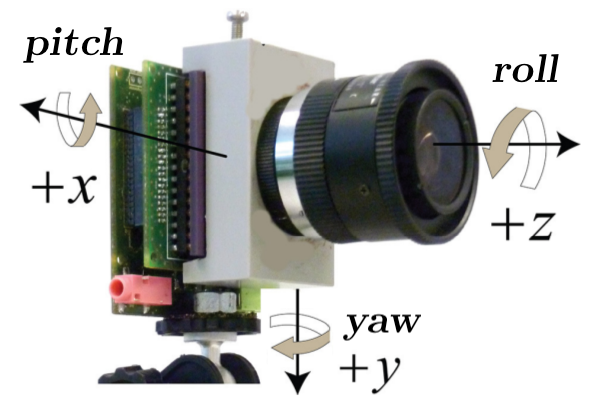
\includegraphics[width = \textwidth]{images/axes.png}
    (a)
  \end{minipage}
  \hfill
  \begin{minipage}[t]{0.48\textwidth}
    \centering 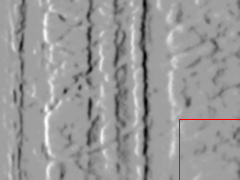
\includegraphics[width =
    \textwidth]{images/slider_groundtruth.png} (b)
  \end{minipage}
  \hfill
  \caption{Axes definition}
  \label{fig:axes}
\end{figure}
\Cref{fig:shapes_6dof_pose} shows the comparison of the results of the
proposed method against ground truth on the whole \textit{shapes\_6dof}
sequence.
\begin{figure}
  \begin{minipage}[t]{\textwidth}
    \centering 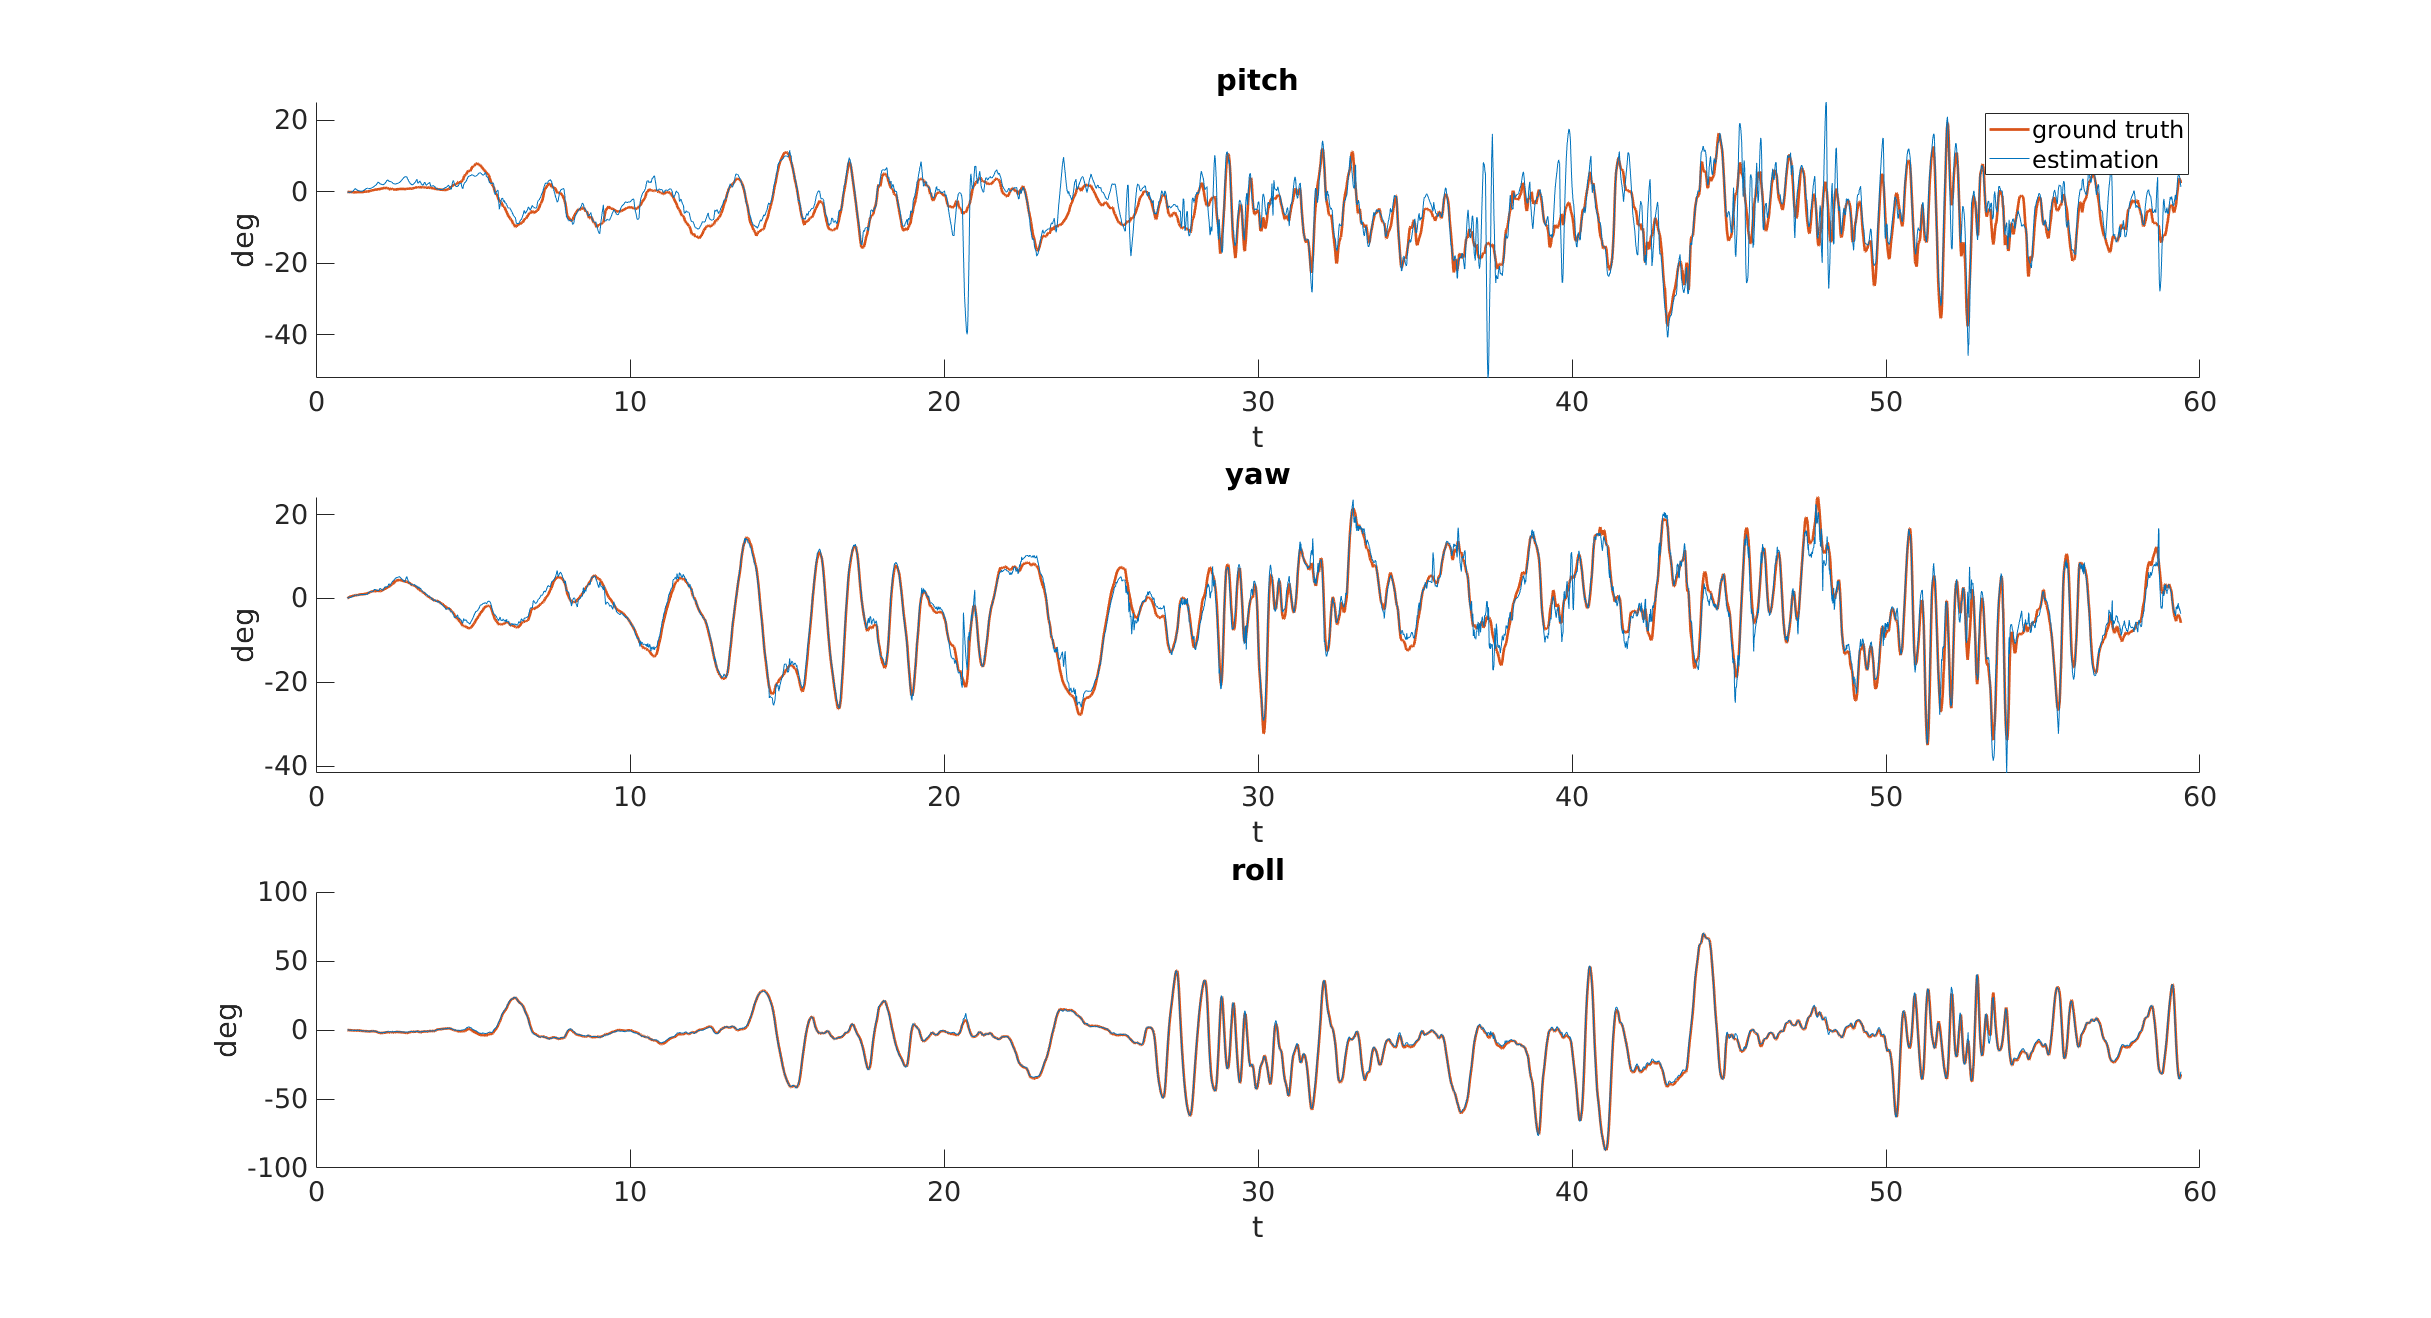
\includegraphics[trim={5cm 0cm 5cm 0cm},clip,width =
    \textwidth]{images/shapes_6dof_rotation.png} (a) Orientation
  \end{minipage}
  \hfill
  \begin{minipage}[t]{\textwidth}
    \centering 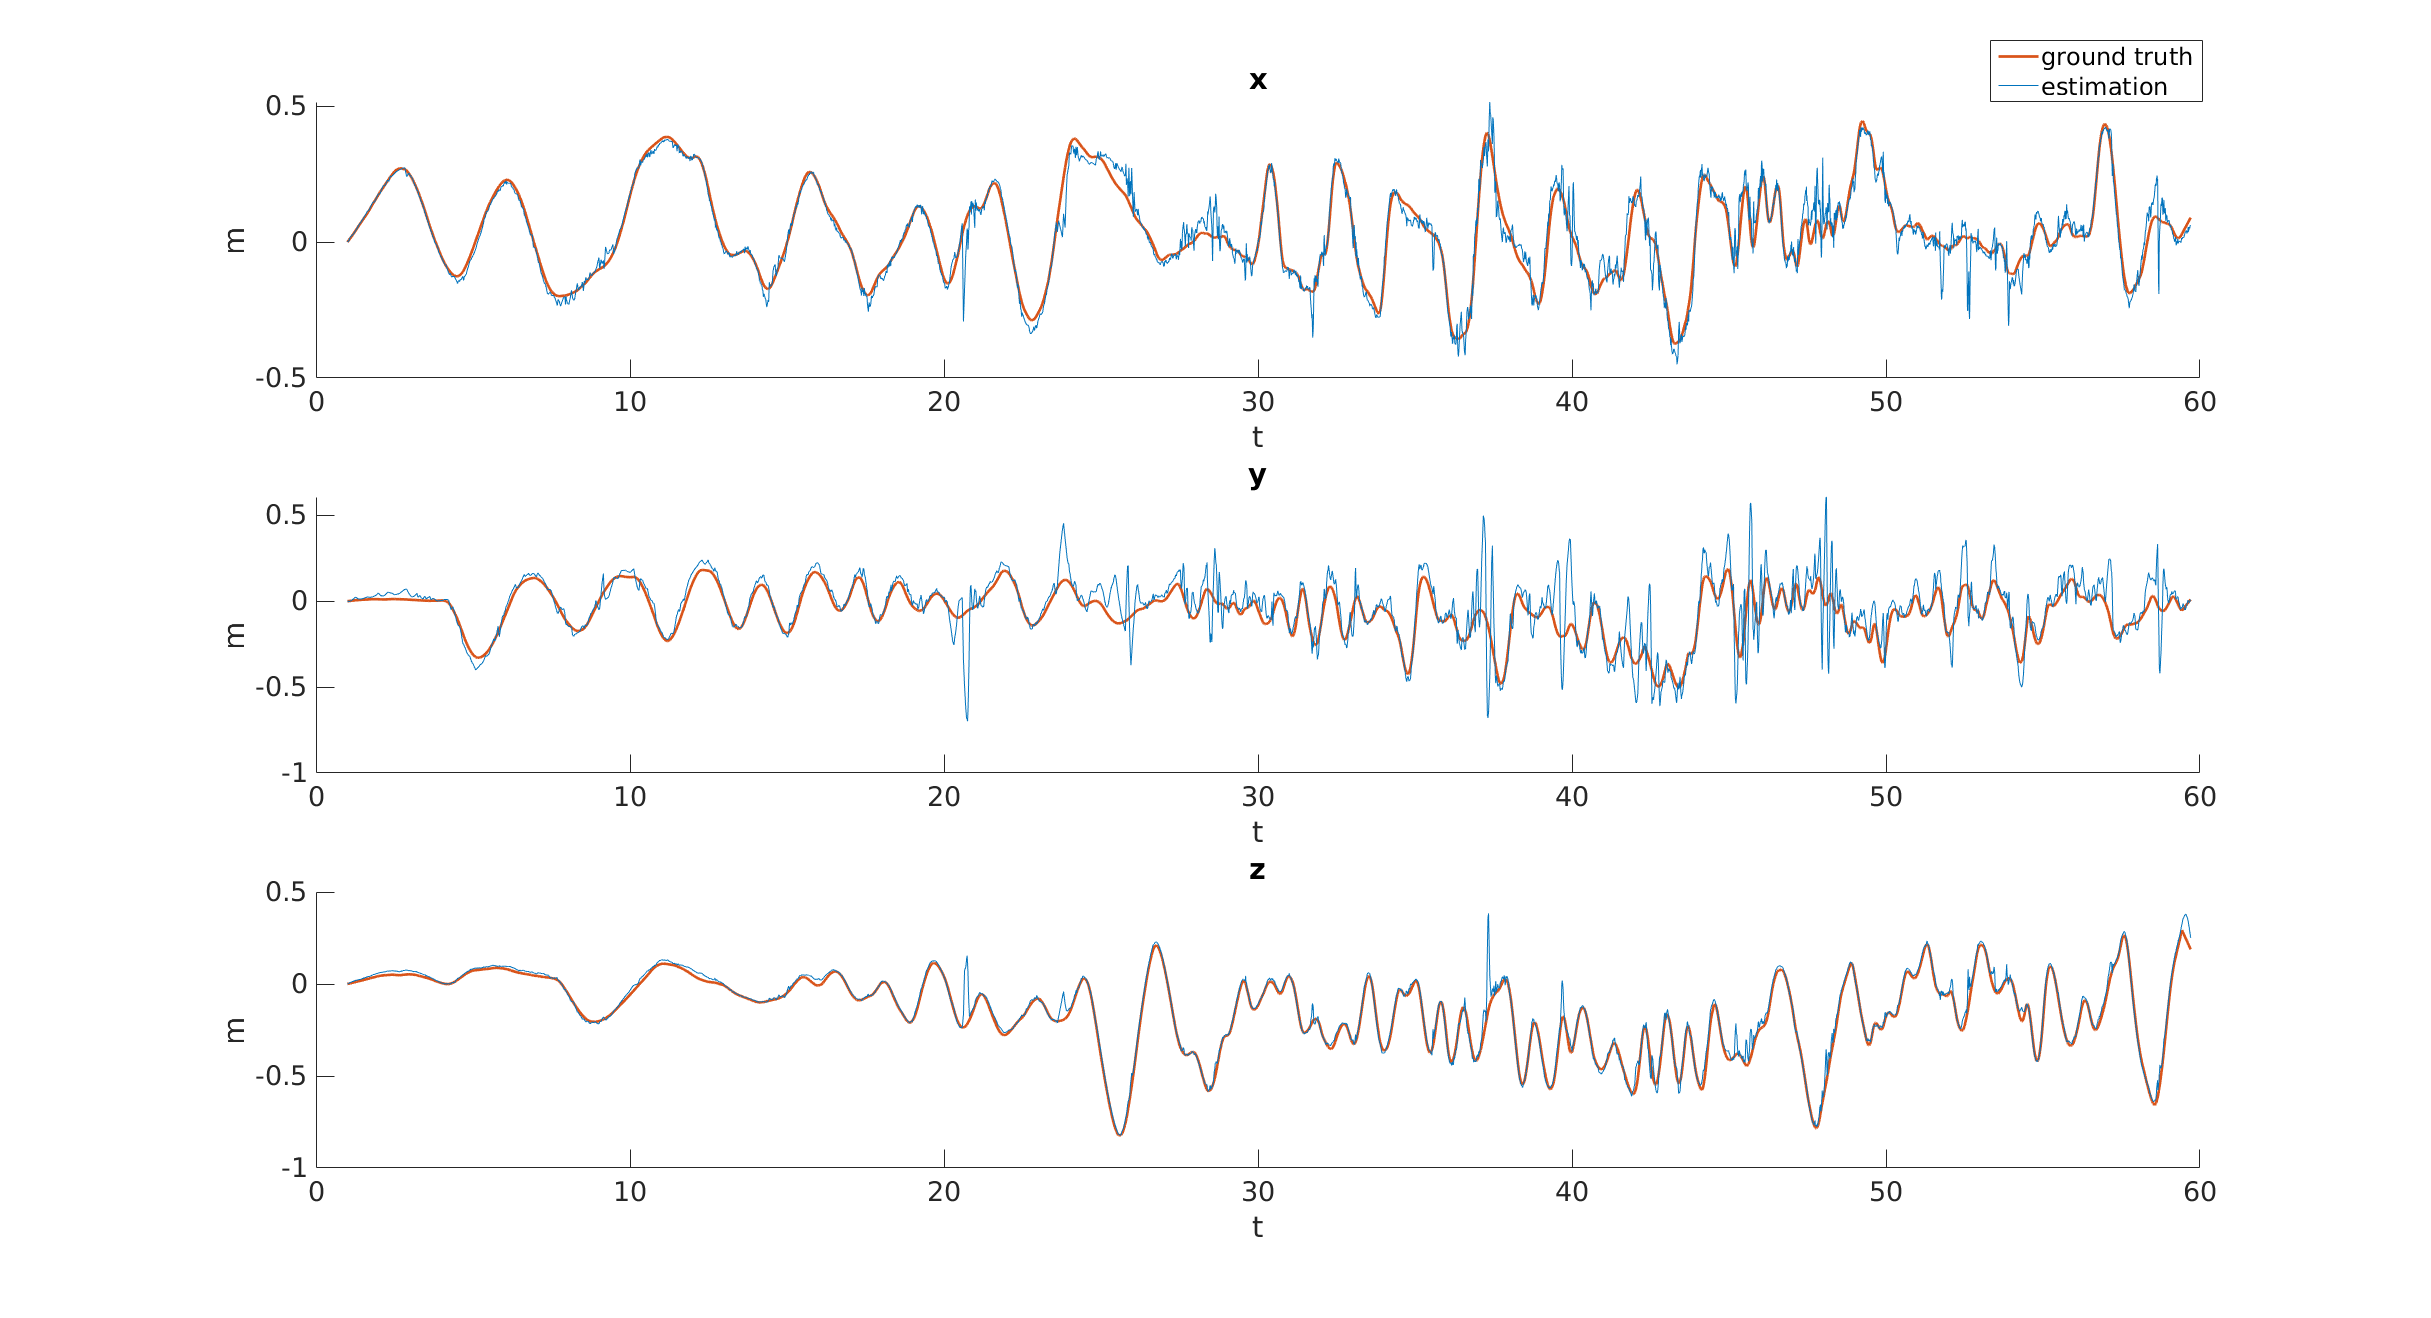
\includegraphics[trim={5cm 0cm 5cm 0cm},clip,width =
    \textwidth]{images/shapes_6dof_translation.png} (b) Translation
  \end{minipage}
  \hfill
  \caption{Axes definition}
  \label{fig:shapes_6dof_pose}
\end{figure}


\begin{table}[h]
\begin{center}
\caption{Quantitative evaluation on planar sequences}\vspace{1ex}
\label{tab:err_est}
\begin{tabular}{l|c|ccc}
\hline
  Dataset &
            \begin{tabular}{c}Mean Orientation\\ Error/deg\\
              \hline
              \begin{tabular}{c|c|c}pitch&yaw&roll\end{tabular}\end{tabular}  &
             \begin{tabular}{c}Mean Translation Error/m\\
              \hline
              \begin{tabular}{c|c|c}x&y&z\end{tabular}\end{tabular} &                                                                 EUDC & NEFZ \\ \hline \hline
shapes\_6dof & s & 780 & 400 & 1180 \\
shapes\_translation & km & 4.052 & 6.955 & 11.007 \\
poster\_6dof& km/h & 18.7 & 62.6 & 33.6 \\
poster\_translation& \% & 36 & 10 & 27 \\
\hline
\end{tabular}
\end{center}
\end{table}

\begin{tabular}{lcccccccl}
\hline
  &\multicolumn{3}{c}{Mean Orientation}& \multicolumn{3}{c}{Mean Translation}&Travelled Distance&Note \\
  Dataset&\multicolumn{3}{c}{Error/deg}& \multicolumn{3}{c}{Error/m}&\\
\cline{2-9}
    & pitch & yaw&roll&x&y&z&46.89& \\
\hline
Gnat      & per gram    & 13.65 &&&&&&     \\
          & each        & 0.01   &&&&&&    \\
Gnu       & stuffed     & 92.50  &&&&&&    \\
Emu       & stuffed     & 33.33   &&&&&&   \\
Armadillo & frozen      & 8.99    &&&&&&   \\
\hline
\end{tabular}

Despite of the rapid movements, in the above datasets the camera
actually only moves in a relative small region in front of the
textured plane, as depicted in \cref{fig:shapes_6dof_path}. However,
this method also applies when camera travels a longer distance with
respect to the scene depth, as shown in
\cref{fig:slider_hdr_far_map}. Also, although this method is designed
for planar scenes, in a complex scene with rotation only movement,
where no scene parameters are needed, this method can still be applied
to build a global map, delivering a result similar to \textit{image
  stitching}. \Cref{fig:boxes_rotation_map} is such an example.
\begin{figure}
  \centering
  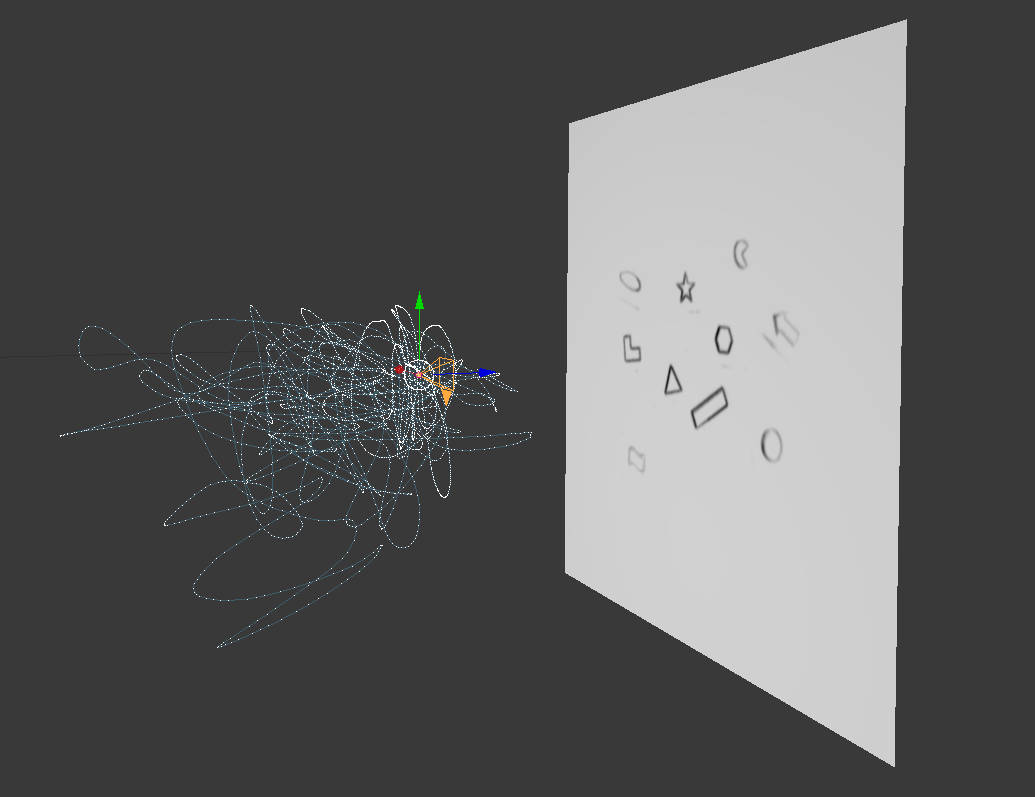
\includegraphics[width=\textwidth]{images/shapes_6dof_path.png}
  \caption{The motion path of the dataset
    \textit{shapes\_6dof}. Despite a trajectory length of about $50m$,
    in the whole $60s$ the camera actually stays in a relative small
    region compared to the scene depth, and there is no observable
    increase of drift using the method in this
    work. \textcolor{red}{ref to error estimation}}
  \label{fig:shapes_6dof_path}
\end{figure}
\begin{figure}
  \centering
  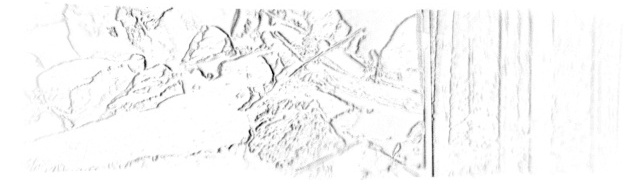
\includegraphics[width=\textwidth]{images/slider_hdr_far_map_36.jpg}
  \caption{The dataset \textit{slider\_hdr\_far}, with a scene depth
    of $0.584 m$, and a camera movement in the positive $x$ direction
    only. Note that this is a much wider map than what we have seen
    before. The figure shows the result at $4.8 sec$ within the whole
    range of $6.3 sec$; afterwards the algorithm is lost in the
    forest, where almost all the textures are vertical, causing severe
    local optima problem. If we constrain the motion estimation to
    translation only, it delivers a much better result.}

  \label{fig:slider_hdr_far_map}
\end{figure}
\begin{figure}
  \centering
  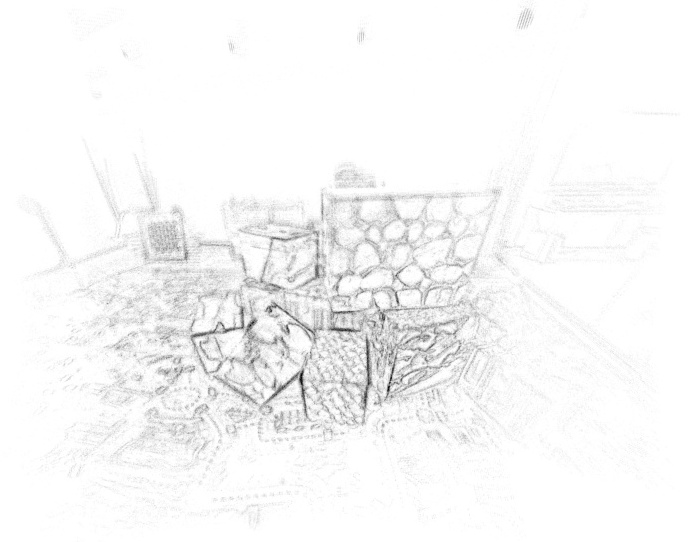
\includegraphics[width=\textwidth]{images/boxes_rotation_map.jpg}
  \caption{The dataset \textit{boxes\_rotation}. The motion in this
    dataset is rotation-dominated}
  \label{fig:boxes_rotation_map}
\end{figure}




\chapter{A Discussion to 6DoF Motion Estimation in General 3D Scenes}
\label{chap:general_scene}



\subsection{note}
\label{sec:note}

tried initialize with multiple frames, didn't work very
well. similarly sliding window didn't work; too many events didn't
work

\chapter{Discussion}
\label{chap:discussion}
One possible reason why the algorithm sometimes get lost is that there
are too few textures available, as shown in
\cref{fig:shapes_tr_lost}(a). At this time we usually need to rely on
the relocalization pipeline. The current implementation of
relocalization needs a good initial guess, so it does not alway work
reliably.
\begin{figure}
  \begin{minipage}[t]{0.48\textwidth}
    \centering 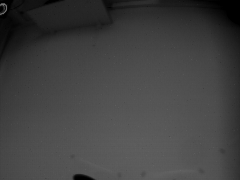
\includegraphics[width =
    \textwidth]{images/frame_00000520.png}
      (a) There is little texture visible
  \end{minipage}
  \hfill
  \begin{minipage}[t]{0.48\textwidth}
    \centering 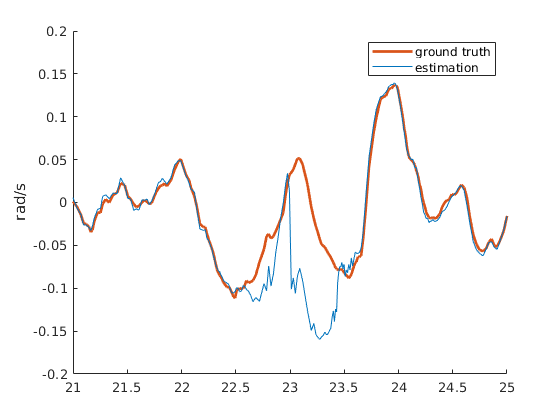
\includegraphics[width =
    \textwidth]{images/shapes_tr_lost.png}
       (b) Relocalized after get lost (roll component)
  \end{minipage}

   \begin{minipage}[t]{0.48\textwidth}
    \centering 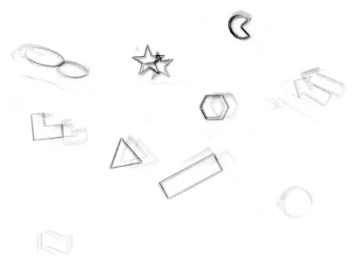
\includegraphics[width =
    \textwidth]{images/map_956.jpg}
     (c) Polluted map after tracking is lost
  \end{minipage} \caption{When tracking the dataset \textit{shapes\_translation}, we
    always get lost at around $23 sec$, where only a small part of the
    oval is visible (a). When later there are more textures available,
    the camera has already moved some distance so that the current
    estimation of the pose might already be far off. The \textit{bundle adjustment }When the
    algorithm confirms that there is little overlap between the
    current frame and the map at this pose. it tries to insert a
    keyframe and track from the new keyframe. The current
    implementation doesn't reinitialize the map after the tracking is
    lost. The advantage is that there is still chance to come back to
    the original map after tracking a wrong ``local map'' (b); the
    disadvantage is that the global map will most likely be polluted
    by the ``local map'' (c)}
  \label{fig:shapes_tr_lost}
\end{figure}



\section{Erstellen einer Tabelle}\label{sec:tabellen}

Ein Beispiel einer Tabelle:
\begin{table}[h]
  \begin{center}
    \caption{Daten der Fahrzyklen ECE, EUDC, NEFZ.}\vspace{1ex}
    \label{tab:tabnefz}
    \begin{tabular}{ll|ccc}
      \hline
      Kennzahl & Einheit & ECE & EUDC & NEFZ \\ \hline \hline
      Dauer & s & 780 & 400 & 1180 \\
      Distanz & km & 4.052 & 6.955 & 11.007 \\
      Durchschnittsgeschwindigkeit & km/h & 18.7 &  62.6 & 33.6 \\
      Leerlaufanteil & \% & 36 & 10 & 27 \\
      \hline
    \end{tabular}
  \end{center}
\end{table}

Die Tabelle wurde erzeugt mit:
\begin{verbatim}
\begin{table}[h]
  \begin{center}
    \caption{Daten der Fahrzyklen ECE, EUDC, NEFZ.}\vspace{1ex}
    \label{tab:tabnefz}
    \begin{tabular}{ll|ccc}
      \hline
      Kennzahl & Einheit & ECE & EUDC & NEFZ \\ \hline \hline
      Dauer & s & 780 & 400 & 1180 \\
      Distanz & km & 4.052 & 6.955 & 11.007 \\
      Durchschnittsgeschwindigkeit & km/h & 18.7 &  62.6 & 33.6 \\
      Leerlaufanteil & \% & 36 & 10 & 27 \\
      \hline
    \end{tabular}
  \end{center}
\end{table}
\end{verbatim}

\section{Weitere nützliche Befehle}\label{sec:div}

Hervorhebungen im Text sehen so aus: \emph{hervorgehoben}. Erzeugt
werden sie mit dem \texttt{\textbackslash epmh\{.\}} Befehl.

Einheiten werden mit den Befehlen \texttt{\textbackslash unit[1]\{m\}}
(z.B.~\unit[1]{m}) und \texttt{\textbackslash unitfrac[1]\{m\}\{s\}}
(z.B.~\unitfrac[1]{m}{s}) gesetzt.
